% !TEX TS-program = pdflatex
% !TEX encoding = UTF-8 Unicode

% This file is a template using the "beamer" package to create slides for a talk or presentation
% - Giving a talk on some subject.
% - The talk is between 15min and 45min long.
% - Style is ornate.

% MODIFIED by Jonathan Kew, 2008-07-06
% The header comments and encoding in this file were modified for inclusion with TeXworks.
% The content is otherwise unchanged from the original distributed with the beamer package.

\documentclass{beamer}

\definecolor{vertmoyen}{HTML}{FFFF00}
\definecolor{vertclair}{HTML}{FFFF00}
\definecolor{vertfonce}{HTML}{FFFF00}
\definecolor{deletecol}{HTML}{FF0000}
\definecolor{addcolor} {HTML}{9E0270}

% Copyright 2004 by Till Tantau <tantau@users.sourceforge.net>.
%
% In principle, this file can be redistributed and/or modified under
% the terms of the GNU Public License, version 2.
%
% However, this file is supposed to be a template to be modified
% for your own needs. For this reason, if you use this file as a
% template and not specifically distribute it as part of a another
% package/program, I grant the extra permission to freely copy and
% modify this file as you see fit and even to delete this copyright
% notice. 


\mode<presentation>
{
  \usetheme{Madrid}
  % or ...

 \usecolortheme{dolphin}

  \setbeamercovered{transparent}
  % or whatever (possibly just delete it)
}


\usepackage[english]{babel}
% or whatever

\usepackage[utf8]{inputenc}
% or whatever

\usepackage{times}
\usepackage[T1]{fontenc}
% Or whatever. Note that the encoding and the font should match. If T1
% does not look nice, try deleting the line with the fontenc.
\usepackage{bussproofs}
\newcommand{\Resolution}[2]{\RightLabel{\footnotesize{$#1$}} \BinaryInfC{$#2$}}

\usepackage[vlined]{algorithm2e}

\usepackage{amsmath}

%\newcommand{\recalltoc}{\frame{\tableofcontents[sectionstyle=show/shaded,subsectionstyle=show/show/hide]}}

\newcommand{\dual}[1]{\ensuremath{\bar{#1}}}
\newcommand{\dn}[2]{#1 \setminus (#2)}
\newcommand{\set}[2]{\ensuremath{\left\{#1\mid#2\right\}}}


\usepackage{tikz}
\usetikzlibrary{positioning}

\tikzstyle{proof edge}=[->,thick,cap=round]
\tikzstyle{deleted edge}=[proof edge, dashed, color=deletecol]

\newcommand{\proofnode}[3][]{
  \node [anchor=mid, #1] (#2) {#3}
}

\newcommand{\rootnode}[1][]{
  \proofnode[#1]{root}{$\bot$}
}

\newcommand<>{\edgewithlabel}[3]{
  \draw#4 [proof edge, color=vertfonce] (#1) -- (#2) node [above, pos=0.3] {\footnotesize #3}
}

\newcommand<>{\drawchildren}[3]{
  \draw#4 [proof edge] (#1) -- (#2);
  \draw#4 [proof edge] (#1) -- (#3)
}

\newcommand{\addchildren}[5]{
  \proofnode[above left  of=#1]{#2}{#3};
  \proofnode[above right of=#1]{#4}{#5}
}

\newcommand{\withchildren}[5]{
  \addchildren{#1}{#2}{#3}{#4}{#5};
  \drawchildren{#1}{#2}{#4}
}

\newcommand<>{\crossnode}[2][]{
  \draw#3 [color=deletecol,thick,cap=round,#1] (#2.mid) ++(10:0.3) -- ++(190:0.6);
}

\newcommand<>{\marknode}[2][.33cm and .29cm]{
  \draw#3 [color=vertclair,line width=1pt] (#2) ellipse (#1);
}
\usepackage{booktabs}
\newenvironment<>{subpart}[1]
{ \begin{block}#2{#1}
  \begin{itemize}
}{
  \end{itemize}
  \end{block}
}


\title[First Order Lower Units] % (optional, use only with long paper titles)
{Towards the Compression of First-Order Resolution Proofs by Lowering Unit Clauses}

%\subtitle{Presentation Subtitle}

\author[Gorzny, Woltzenlogel Paleo] % (optional, use only with lots of authors)
{J. Gorzny\inst{1} \and B. Woltzenlogel Paleo\inst{2}}
% - Use the \inst{?} command only if the authors have different
%   affiliation.

\institute[] % (optional, but mostly needed)
{
  \inst{1}%
  University of Victoria
  \and
  \inst{2}%
  Vienna University of Technology}
% - Use the \inst command only if there are several affiliations.
% - Keep it simple, no one is interested in your street address.

\date[CADE15] % (optional)
{6 August 2015}

%\subject{Talks}
% This is only inserted into the PDF information catalog. Can be left
% out. 



% If you have a file called "university-logo-filename.xxx", where xxx
% is a graphic format that can be processed by latex or pdflatex,
% resp., then you can add a logo as follows:

% \pgfdeclareimage[height=0.5cm]{university-logo}{university-logo-filename}
% \logo{\pgfuseimage{university-logo}}



% Delete this, if you do not want the table of contents to pop up at
% the beginning of each subsection:
%\AtBeginSubsection[]
%{
%  \begin{frame}<beamer>{Outline}
%    \tableofcontents[currentsection,currentsubsection]
%  \end{frame}
%}


% If you wish to uncover everything in a step-wise fashion, uncomment
% the following command: 

%\beamerdefaultoverlayspecification{<+->}


\begin{document}
\def\e{\mbox{\ $\vdash$\ }}

\begin{frame}
  \titlepage
\end{frame}

%\begin{frame}{Outline}
%  \tableofcontents
  % You might wish to add the option [pausesections]
%\end{frame}


% Since this a solution template for a generic talk, very little can
% be said about how it should be structured. However, the talk length
% of between 15min and 45min and the theme suggest that you stick to
% the following rules:  

% - Exactly two or three sections (other than the summary).
% - At *most* three subsections per section.
% - Talk about 30s to 2min per frame. So there should be between about
%   15 and 30 frames, all told.

\section{Introduction}

%\subsection[Short First Subsection Name]{First Subsection Name}

\begin{frame}{Proof Compression Motivation}
an accessible, good motivational example for proof compression
\end{frame}

\begin{frame}{(Propositional) Proofs}
%introduction to proofs as we're going to see them, ideally formally and with a small example

\begin{definition}[Proof]
A directed acyclic graph $\langle V,E,\Gamma \rangle$, where
\begin{itemize}
\item $V$ is a set of nodes
\item $E$ is a set of edges labeled by literals
\item $\Gamma$ (the proof clause) is inductively constructible using \emph{axiom} and \emph{resolution} nodes
\end{itemize}
\end{definition}

\begin{definition}[Axiom]
A proof with a single node (so $E=\emptyset$)
\end{definition}
\end{frame}

\begin{frame}{(Propositional) Resolution}
%a quick introduction to resolution, with a small propositional example
\begin{definition}[Resolution]
Given two proofs $\psi_L$ and $\psi_R$ with conclusions $\Gamma_L$ and $\Gamma_R$ with some literal $l$ such that $\overline{l}\in \Gamma_L$ and $l\in \Gamma_R$, the resolution proof $\psi$ of $\psi_L$ and $\psi_R$ on $l$, denoted $\psi=\psi_L \psi_R$ is such that:
\begin{itemize}
\item $\psi$'s nodes are the union of the nodes of $\psi_L$ and $\psi_R$, and a new root node
\item there is an edge from $\rho(\psi)$ to $\rho(\psi_L)$ labeled with $\overline{l}$
\item there is an edge from $\rho(\psi)$ to $\rho(\psi_R)$ labeled with $l$
\item $\psi$'s conclusion is $(\Gamma_L\setminus\{\overline{l}\})\cup(\Gamma_R\setminus\{l\})$
\end{itemize}
\end{definition}
\end{frame}

\begin{frame}{A Propositional Proof}
%a small example to illustrate the definitions from the last two slides\\
%the example should be redundant, so that we can show it again after the next slide in it's more minimal state\\
%ideally minimized via LU, so that we can show the transformation later
      \centering
      \begin{tikzpicture}[node distance=1.2cm]
        \rootnode;
        \withchildren{root} {r9}{\dual{c}}  {r6}{c};
     \proofnode[above left of=r9] {r8} {a,\dual{c}};
     \proofnode[above of=r8] {r7} {a,\dual{b},\dual{c}};
     \proofnode[above right of=r6] {r5} {a,c};

        \withchildren{r5}  {r4}{b} {r2}{a,\dual{b},c};
        \withchildren{r4}   {r1}{\dual{a}} {r3}{a,b};
        \drawchildren {r6} {r1} {r5};
      \draw[proof edge] (r9) -- (r1);
      \draw[proof edge] (r9) -- (r1);
      \draw[proof edge] (r9) -- (r8);
      \draw[proof edge] (r8) -- (r7);
      \draw[proof edge] (r8) -- (r4);
      \end{tikzpicture}
\end{frame}


\begin{frame}{Deletion}
how deleting subproofs or edges in proofs affect them
\end{frame}

\begin{frame}{Redundancy}
types of redundancy we hope to remove, small examples (before/after proofs; not animated)
\end{frame}

\begin{frame}{First-Order Proofs}
%key differences from propositional case; example of first order proofs
\begin{definition}[First-Order Proof]
A directed acyclic graph $\langle V,E,\Gamma \rangle$, where
\begin{itemize}
\item $V$ is a set of nodes
\item $E$ is a set of edges labeled by literals {\bf and substitutions}
\item $\Gamma$ (the proof clause) is inductively constructible using \emph{axiom}, {\bf\emph{(first order) resolution}}, {\bf and \emph{contraction}} nodes
\end{itemize}
\end{definition}

Axioms are unchanged
\end{frame}

\begin{frame}{Substitutions and Unifiers}
\begin{definition}[Substitution]
A mapping $\{X_1\setminus t_1, X_2\setminus t_2,\ldots\}$ from variables $X_1,X_2,\ldots$ to terms $t_1,t_2,\ldots$
\end{definition}

%example here

\begin{definition}[Unifier]
%A set of literals in a substitution that makes all literals in the set equal
\end{definition}

%example here
\end{frame}

\begin{frame}{First Order (Unifying) Resolution}
%definition (incl. mgu); ?
%example of unifying resolution ?
\begin{definition}[First Order Resolution]
Given two proofs $\psi_L$ and $\psi_R$ with conclusions $\Gamma_L$ and $\Gamma_R$ with some literal $l$ such that $l_L\in \Gamma_L$ and $l_R\in \Gamma_R$, and $\sigma_L$ and $\sigma_R$ are substitutions usch that $l_L\sigma_L=\overline{l_R}\sigma_R$, and the variables in $(\Gamma_L\setminus l_L)\sigma_L$ and $(\Gamma_R\setminus l_R)\sigma_R$ are disjoint, then the resolution proof $\psi$ of $\psi_L$ and $\psi_R$ on $l$, denoted $\psi=\psi_L \psi_R$ is such that:
\begin{itemize}
\item $\psi$'s nodes are the union of the nodes of $\psi_L$ and $\psi_R$, and a new root node
\item there is an edge from $\rho(\psi)$ to $\rho(\psi_L)$ labeled with $l_L$ and $\sigma_L$
\item there is an edge from $\rho(\psi)$ to $\rho(\psi_R)$ labeled with $l_R$ and $\sigma_R$
\item $\psi$'s conclusion is $(\Gamma_L\setminus l_L)\sigma_L\cup (\Gamma_R\setminus l_R)\sigma_R$
\end{itemize}
\end{definition}
\end{frame}

\begin{frame}{Contraction}
%definition; small example
\begin{definition}[Contraction]
If $\psi'$ is a proof and $\sigma$ is a unifier of $\{l_1,\ldots,l_n\}\subset \Gamma'$, then a contraction $\psi$ is a proof where
\begin{itemize}
\item $\psi$'s nodes are the union of the nodes of $\psi'$ and a new node $v$
\item There is an edge from $\rho(\psi')$ to $v$ labeled with $\{l_1,\ldots,l_n\}$ and $\sigma$
\item The conclusion is $(\Gamma'\setminus \{l_1,\ldots,l_n\})\sigma \cup \{l\}$, where $l=l_k\sigma$ for $k\in \{1,\ldots,n\}$
\end{itemize}
\end{definition}
\end{frame}

\section{Propositional Algorithm}

\begin{frame}{LowerUnits}
brief high level description; complexity\\
probably not pseudo-code
\end{frame}

\begin{frame}{Propositional Example}
%quick, clear example of LU (animated), perhaps showing how one of the redundancies described before is fixed
\begin{columns}
\column{0.5\textwidth}
      \begin{center}
      \begin{tikzpicture}[node distance=1.2cm]
        \rootnode;
        \withchildren{root} {r9}{\dual{c}}  {r6}{c};
     \proofnode[above left of=r9] {r8} {a,\dual{c}};
     \proofnode[above of=r8] {r7} {a,\dual{b},\dual{c}};
     \proofnode[above right of=r6] {r5} {a,c};
      \draw[proof edge] (r9) -- (r1);
        \withchildren{r5}  {r4}{b} {r2}{a,\dual{b},c};
        \withchildren{r4}   {r1}{\dual{a}} {r3}{a,b};
        \drawchildren {r6} {r1} {r5};
      \draw[proof edge] (r9) -- (r1);
      \draw[proof edge] (r9) -- (r8);
      \draw[proof edge] (r8) -- (r7);
      \draw[proof edge] (r8) -- (r4);
      \end{tikzpicture}
\end{center}
\column{0.5\textwidth}
  \only<1-3>{
      \begin{center}
      \begin{tikzpicture}[node distance=1.2cm]
 \proofnode {root}{\alt<3>{a,\dual{b}}{$\bot$}};
%        \withchildren{root} {r9}{\dual{c}}  {r6}{c};
 \proofnode[above right of=root] {r6}{c};
 \proofnode[above left of=root] {r9}{\dual{c}};
     \proofnode[above right of=r6] {r5} {a,c};
     \proofnode[above right of=r5] {r2} {a,\dual{b},c};
     \proofnode[above left of=r5] {r4} {b};
     \proofnode[above left of=r4] {r1} {\dual{a}};
     \proofnode[above right of=r4] {r3} {a,b};
     \proofnode[above left of=r9] {r8} {a,\dual{c}};
     \proofnode[above of=r8] {r7} {a,\dual{b},\dual{c}};

\marknode<2>{r4};
\marknode<2->{r1};
\marknode<3>{r3};

      \draw<-1>[proof edge] (r9) -- (r1);
      \draw<-1>[proof edge] (r9) -- (r8);
      \draw<-1>[proof edge] (r8) -- (r7);
      \draw<-1>[proof edge] (r8) -- (r4);
      \draw<-2>[proof edge] (root) -- (r6);
      \draw<-2>[proof edge] (root) -- (r9);
      \draw<-1>[proof edge] (r6) -- (r1);
      \draw<-1>[proof edge] (r6) -- (r5);
      \draw<-1>[proof edge] (r5) -- (r4);
      \draw<-1>[proof edge] (r5) -- (r2);
      \draw<-1>[proof edge] (r4) -- (r1);
      \draw<-1>[proof edge] (r4) -- (r3);

      \draw<2>[deleted edge] (r9) -- (r1);
      \draw<-2>[proof edge] (r9) -- (r8);
      \draw<-2>[proof edge] (r8) -- (r7);
      \draw<2>[deleted edge] (r8) -- (r4);
      \draw<2>[deleted edge] (r6) -- (r1);
      \draw<-2>[proof edge] (r6) -- (r5);
      \draw<2>[deleted edge] (r5) -- (r4);
      \draw<-2>[proof edge] (r5) -- (r2);
      \draw<2>[deleted edge] (r4) -- (r1);
      \draw<2>[proof edge] (r4) -- (r3);

%      \draw<3>[proof edge] (r4) -- (r3);
      \draw<3>[proof edge] (root) .. controls (r9.north east) .. (r7);
      \draw<3>[proof edge] (root) .. controls (r5.north west) .. (r2);

\crossnode<3>{r9}
\crossnode<3>{r4}
\crossnode<3>{r6}
\crossnode<3>{r8}
\crossnode<3>{r5}
      \draw<3>[deleted edge] (r4) -- (r3);

%        \drawchildren {r6} {r1} {r5};

%      \draw<2->[deleted edge] (r1) -- (r6);
%      \draw<-3>[proof edge] (r9) -- (r6);
%      \draw<4>[deleted edge] (r9) -- (r6);
      \end{tikzpicture}
\end{center}
}
  \only<4->{
      \begin{center}
      \begin{tikzpicture}[node distance=1.2cm]
     \proofnode{n2} {\alt<6->{$\bot$}{}};
     \proofnode [above left of=n2]{n1} {\alt<5->{a}{}};
     \proofnode [above right of=n2]{n3} {\alt<6->{\dual{a}}{}};
     \proofnode [above right of=n1]{n4} {\alt<5->{a,b}{}};
 \proofnode [above left of=n1]{root}{\alt<3->{a,\dual{b}}{$\bot$}};
     \proofnode[above right of=root] {r2} {a,\dual{b},c};
     \proofnode[above left of=root] {r7} {a,\dual{b},\dual{c}};

      \draw<4->[proof edge] (root) --  (r7);
      \draw<4->[proof edge] (root) -- (r2);
\marknode<5>{n4};
\marknode<6>{n3};
      \draw<5->[proof edge] (n1) -- (root);
      \draw<5->[proof edge] (n1) -- (n4);
      \draw<6->[proof edge] (n2) -- (n1);
      \draw<6->[proof edge] (n2) -- (n3);
      \end{tikzpicture}
\end{center}
}
\end{columns}
\end{frame}

\section{First-Order Algorithm}

\begin{frame}{First Order Change: Helpful Contractions}
\begin{columns}
\column{0.5\textwidth}
      \begin{center}
      \begin{tikzpicture}[node distance=2cm]
     \proofnode {root} {$\bot$};
     \proofnode[above right of=root] {n5} {$\eta_5$: $p(X)\e$};
 \proofnode[above left of=n5] {n3} {$\eta_3$: $\e q(Z)$};
 \proofnode[above right of=n5] {n4} {$\eta_4$: $p(X), q(Z)\e$};
 \proofnode[above right of=n3] {n1} {$\eta_1$: $p(W)\e q(Z)$};
 \proofnode[above left of=n3] {n2} {$\eta_2$: $\e p(Y)$};
      \draw[proof edge] (root) .. controls (n3.south west) ..  (n2);
      \draw[proof edge] (root) -- (n5);
      \draw[proof edge] (n5) -- (n3);
      \draw[proof edge] (n5) -- (n4);
      \draw[proof edge] (n3) -- (n1);
      \draw[proof edge] (n3) -- (n2);
\marknode<2->{n2};
      \end{tikzpicture}
\end{center}
\column{0.5\textwidth}
\begin{center}
\only<3->{
      \begin{tikzpicture}[node distance=2cm]
     \proofnode {n5} {$\eta_5': p(X),p(Y)\e$};
 \proofnode[above right of=n5] {n4} {$\eta_4'$: $p(X),q(Z)\e $};
 \proofnode[above left of=n5] {n1} {$\eta_1'$: $p(W)\e q(Z)$};
 \proofnode[below left of=n5] {n5c} {\alt<4->{$\lfloor\eta_5'\rfloor$: $p(U)\e$}{}};
 \proofnode[below right of=n5] {n2} {\alt<5->{$\eta_2'$: $\e p(Y)$}{}};
 \proofnode[below right of=n5c] {root} {\alt<5->{$\bot$}{}};
      \draw[proof edge] (n5) -- (n1);
      \draw[proof edge] (n5) -- (n4);
      \draw<4->[proof edge] (n5c) -- (n5);
      \draw<5->[proof edge] (root) -- (n2);
      \draw<5->[proof edge] (root) -- (n5c);

      \end{tikzpicture}
}
\end{center}
\end{columns}

\end{frame}

\begin{frame}{First Order Challenge: Pre-Deletion Check}
%example 2 demonstrated; definition of pre-deletion unification property
%\begin{columns}
%\column{0.5\textwidth}
\begin{center}
      \begin{tikzpicture}[node distance=2cm]
     \proofnode {root} {$\bot$};
 \proofnode[above right of=root] {n2} {$\eta_2$: $\e q(Y)$};
 \proofnode[above left of=root] {n1} {$\eta_1$: $q(Y) \e$};
 \proofnode[above left of=n1] {n5} {$\eta_5$: $q(Y) \e p(a)$};
 \proofnode[above right of=n1] {n4} {$\eta_4$: $p(X) \e $};
 \proofnode[above right of=n2] {n3} {$\eta_3$: $\e p(b),q(Y) $};
      \draw[proof edge] (root) -- (n1);
      \draw[proof edge] (root)  -- (n2);
      \draw[proof edge] (n1) -- (n5);
      \draw[proof edge] (n1) -- (n4);
      \draw[proof edge] (n2) -- (n4);
      \draw[proof edge] (n2) -- (n3);
\marknode<2->{n4};
      \end{tikzpicture}\\
%\vspace{3cm}
%\end{center}
%\column{0.5\textwidth}
%\begin{center}
%\vspace*{2cm}
\only<3-4>{
      \begin{tikzpicture}[node distance=2.25cm]
     \proofnode {root} {$\eta$: $\e p(a),p(b)$};
 \proofnode[above left of=root] {n5} {$\eta_5'$: $q(Y) \e p(a)$};
 \proofnode[above right of=root] {n3} {$\eta_3'$: $\e p(b),q(Y) $};
 \proofnode[below=0.5 of root] {n} {\alt<4->{$\lfloor\eta \rfloor$}{}};
      \draw[proof edge] (root) -- (n5);
      \draw[proof edge] (root) -- (n3);
\draw<4->[proof edge] (n) -- (root);
\crossnode<4->{n}
      \end{tikzpicture}
}
\only<5->{
\begin{definition}[Pre-Deletion Property]
$\eta$ unit, $l\in \eta$, such that $l$ is resolved with literals $l_1,\ldots,l_n$ in a proof $\psi$. $\eta$ satisfies the \emph{pre-deletion unifiability} property in $\psi$ if $l_1,\ldots,l_n$ and $\overline{l}$ are unifiable.
\end{definition}
}
\end{center}
%\end{columns}

\end{frame}

\begin{frame}{First Order Challenge: Post-Deletion Check}
%example 3 demonstrated; definition of post-deletion unification property
\begin{center}
      \begin{tikzpicture}[node distance=2.5cm]

     \proofnode {root} {$\bot$};
% \proofnode[above right=0.5cm and 0.05cm of root] {n5} {$\eta_5$: $p(U,q(W,b)) \e$};
% \proofnode[above left=0.5cm and 0.05cm of n5] {n3} {$\eta_3$: $r(V),p(U,q(V,b)) \e$};
% \proofnode[above right=0.5cm and 1pt of n5] {n4} {$\eta_4$: $\e r(W)$};
% \proofnode[above right=0.5cm and 0.05cm of n3] {n1} {$\eta_1$: $r(Y),p(X,q(Y, b)),p(X,Y)\e $};
% \proofnode[above left=0.5cm and 0.05cm of n3] {n2} {$\eta_2$: $\e p(U,V)$};
 \proofnode[above left=0.25cm of root] {n5} {$\eta_5$: $p(U,q(W,b)) \e$};
 \proofnode[above right=0.25cm and -2cm of n5] {n3} {$\eta_3$: $r(V),p(U,q(V,b)) \e$};
 \proofnode[above left=0.25cm and -1cm of n5] {n4} {$\eta_4$: $\e r(W)$};
 \proofnode[above left=0.25cm and -2cm of n3] {n1} {$\eta_1$: $r(Y),p(X,q(Y, b)),p(X,Y)\e $};
 \proofnode[above right=0.25cm and -1cm of n3] {n2} {$\eta_2$: $\e p(U,V)$};
      \draw[proof edge] (root) .. controls (n3.south east) .. (n2);
      \draw[proof edge] (root) -- (n5);
      \draw[proof edge] (n5) -- (n4);
      \draw[proof edge] (n5) -- (n3);
      \draw[proof edge] (n3) -- (n2);
      \draw[proof edge] (n3) -- (n1);
\marknode<2->{n1};
      \end{tikzpicture}\\
\only<3-4>{
\vspace{0.5cm}
      \begin{tikzpicture}[node distance=1.5cm]
 \proofnode {n5} {$\eta_5'$: $p(X,q(W,b)), p(X,W) \e$};
 \proofnode[above left of=n5] {n1} {$\eta_1'$: $r(Y),p(X,q(Y, b)),p(X,Y)\e $};
 \proofnode[right=1cm of n1] {n4} {$\eta_4'$: $\e r(W)$};
 \proofnode[below=0.5cm of n5] {n} {\alt<4->{$\lfloor \eta_5'\rfloor$}{}};

      \draw[proof edge] (n5) -- (n1);
      \draw[proof edge] (n5) -- (n4);
      \draw<4->[proof edge] (n) -- (n5);
\crossnode<4->{n}

      \end{tikzpicture}
}
\only<5->{
\begin{definition}[Post-Deletion Property]
$\eta$ unit, $l\in \eta$, such that $l$ is resolved with literals $l_1,\ldots,l_n$ in a proof $\psi$. $\eta$ satisfies the \emph{post-deletion unifiability} property in $\psi$ if $l_1^{\dagger\downarrow},\ldots,l_n^{\dagger\downarrow}$ and $\overline{l^\dagger}$ are unifiable, where $l^\dagger$ is the literal in $\psi'=\psi\setminus\{\eta\}$ corresponding to $l$ in $\psi$, and $l^{\dagger\downarrow}$ is the descendant of $l^\dagger$ in the roof of $\psi'$.
\end{definition}
}
\end{center}
\end{frame}

\begin{frame}{First Order Lower Units Ideas/Principles}
briefly mention all ideas, e.g. quadratic time naive approach to deal with both properties
\end{frame}

\begin{frame}{Simple/Greedy First Order Lower Units}
introduce simpler idea, make compromises explicit and list benefits\\
high level description\\
(probably not pseudo-code, but list \# of traversals, complexity, etc)
\end{frame}

\begin{frame}{First Order Example}
small, animated example
\end{frame}

\section{Experiment Results}

\begin{frame}{Experiment Setup}
%  \begin{subpart}{Configuration (Simple First Oder Lower Units)}
\begin{itemize}
\item Simple First Order Lower units implemented as part of Skeptik (in Scala)
\end{itemize}

\begin{itemize}
    \item 308 real first-order proofs generated by SPASS from problems from TPTP Problem Library
    \item proofs \emph{generated} on cluster at the University of Victoria
    \item proofs \emph{compressed} on \emph{this laptop}
\end{itemize}
\vspace{1cm}
\pause
\begin{center}
Time to generate proofs: $\approx 40$ minutes\\
Time to compress proofs: \alert{$\approx 5$ seconds} 
\end{center}
%  \end{subpart}
\end{frame}

\begin{frame}{Results}
%at least one or two of the more informative graphs
\begin{columns}
\column{0.5\textwidth}
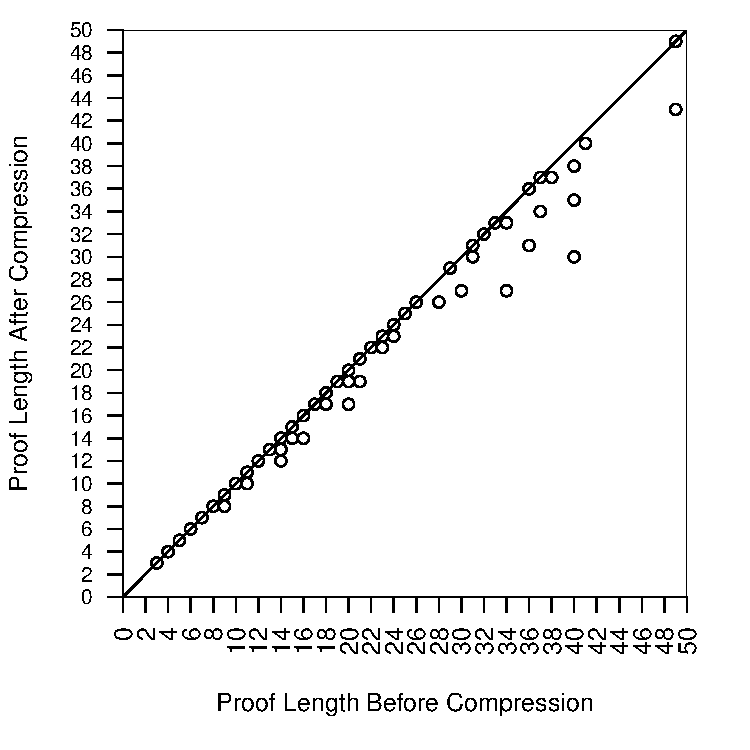
\includegraphics[scale=0.5]{images/compress_length_no_sub_vs_length_all_proofs.pdf}
\column{0.5\textwidth}
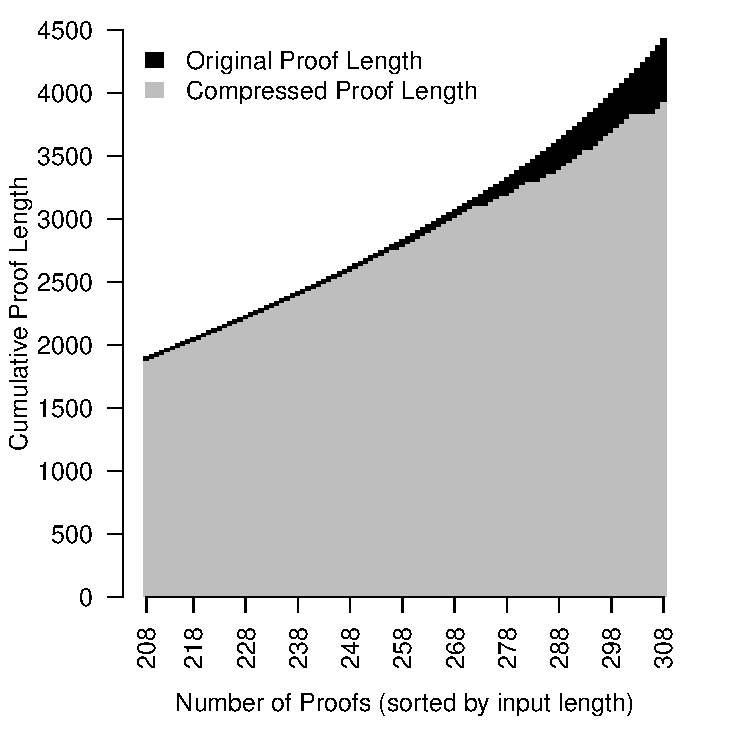
\includegraphics[scale=0.5]{images/cumulative_res_nodes_no_subs_top100.pdf}
%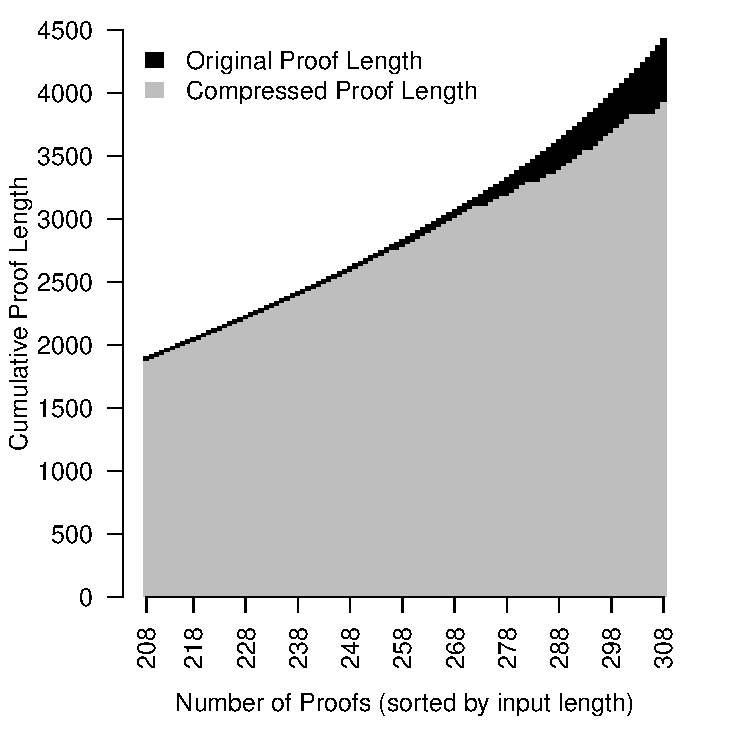
\includegraphics[scale=0.5]{images/cumulative_res_nodes_no_subs_top100.pdf}
%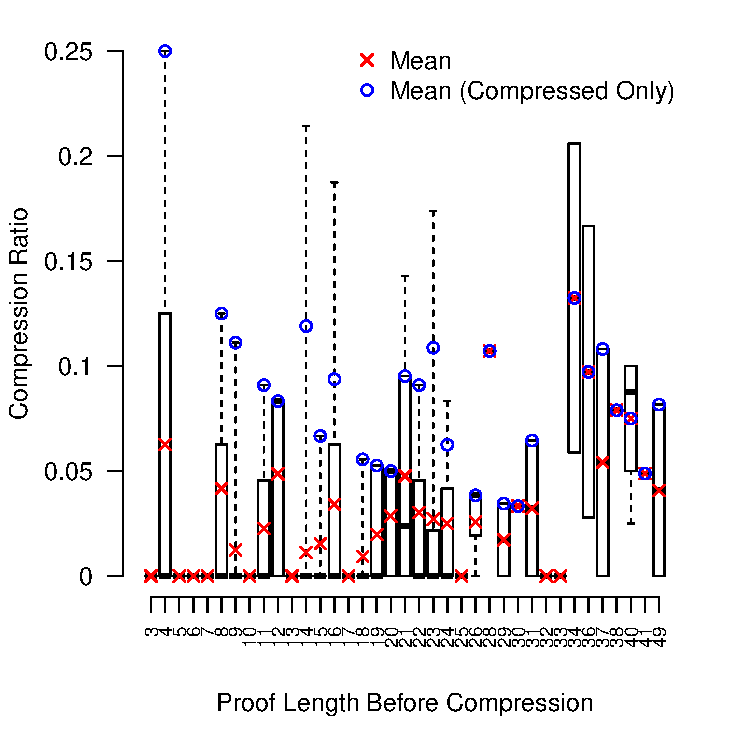
\includegraphics[scale=0.5]{images/compress_ratio_res_vs_proof_length_all_proofs.pdf}
%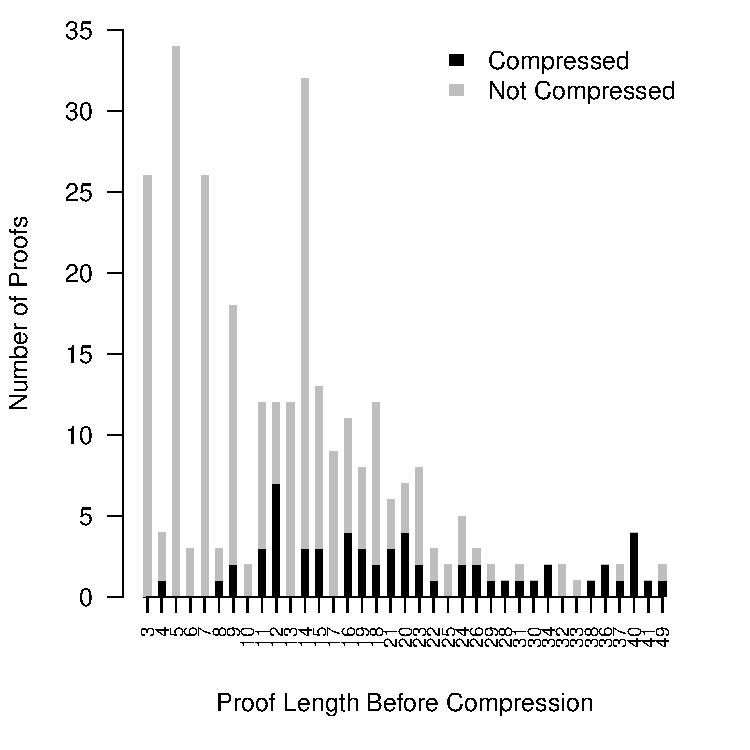
\includegraphics[scale=0.5]{images/num_compressed_stacked.pdf}
%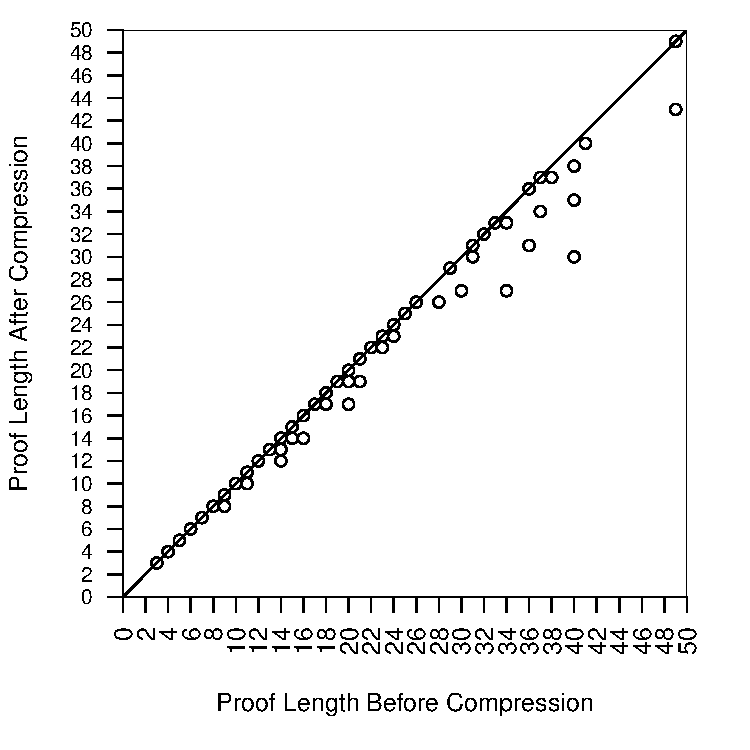
\includegraphics[scale=0.5]{images/compress_length_no_sub_vs_length_all_proofs.pdf}
\end{columns}
\end{frame}

\begin{frame}{Results}
%text summary of results (numbers, percentages, times, etc)
Higher compression in longer proofs: 13/18 proofs with length $\ge 30$ nodes successfully compressed.\\
\vspace{1cm}
Total compression ratio \alert{11.3\%}: 4429 vs. 3929 nodes.\\
\hspace{1cm}\alert{18.4\%} for 100 longest proofs.
\vspace{1cm}

\end{frame}

\section*{Summary}

\begin{frame}{Conclusion}
\begin{itemize}
\item Simple First Order Lower Units is a quick algorithm for first order proof compression
\item Future work:
\begin{itemize}
\item Explore other proof compression algorithms, e.g. Recycle Pivots with Intersection
\item Explore ways of dealing with the post-deletion property quickly
\end{itemize}
\end{itemize}



\begin{center}
\alert{Thank you for your attention.\\
Any questions?}
\end{center}
\footnotesize{
\begin{itemize}
\item Source code: \url{https://github.com/jgorzny/Skeptik}
\item Data: \url{http://www.math.uvic.ca/~jgorzny/data/}
\end{itemize}
}
\end{frame}


\end{document}


